\documentclass[parskip=full]{scrartcl}
\usepackage[utf8]{inputenc} % use utf8 file encoding for TeX sources 

\usepackage[T1]{fontenc} % avoid garbled Unicode text in pdf 
\usepackage[german]{babel} % german hyphenation, quotes, etc 
\usepackage{hyperref} % detailed hyperlink/pdf configuration
\usepackage{graphicx}
\usepackage[toc]{glossaries}
\usepackage{caption}
\usepackage{pdfpages}
\hypersetup{ % ‘texdoc hyperref‘ for options 
	pdftitle={Entwurf}, %
	bookmarks=true,%
}
\usepackage{csquotes} % provides \enquote{} macro for "quotes"
\usepackage{enumitem}
\makeglossaries



\newglossaryentry{GUI}
{
	name={GUI},
	description={Graphical User Interface. Die grafische Benutzeroberfläche}
}
\newglossaryentry{REST}
{
	name={REST},
	description={REST steht für Representational State Transfer und ist ein Programmierparadigma. \href{https://de.wikipedia.org/wiki/Representational_State_Transfer}{https://de.wikipedia.org/wiki/Representational\_State\_Transfer}}
}
\newglossaryentry{URL}
{
	name={URL},
	description={Ein Uniform Resource Locator (Abgekürzt URL) identifiziert eine Ressource.
		\href{https://de.wikipedia.org/wiki/Uniform_Resource_Locator}{https://de.wikipedia.org/wiki/Uniform\_Resource\_Locator}}
}
\newglossaryentry{WS}
{
	name={WebSocket},
	description={Ein auf TCP basierendes Netzwerkprotokoll. \href{https://de.wikipedia.org/wiki/WebSocket}{https://de.wikipedia.org/wiki/WebSocket}}
}
\newglossaryentry{HTTP}
{
	name={HTTP},
	description={Das Hypertext Transfer Protcol ist ein Protokoll zur Übertragung von Daten auf der Anwendungsschicht. Wird meistens zum laden von Websiten verwendet. \href{https://de.wikipedia.org/wiki/Hypertext_Transfer_Protocol}{https://de.wikipedia.org/wiki/Hypertext\_Transfer\_Protocol}}
}

\begin{document}
	\begin{titlepage}
			
		\centering
		\vspace*{0.2\textheight}
		{\Large Praxis der Softwareentwicklung}\\[\baselineskip]
		\vspace{2cm}
		{\Huge \textbf{Entwurf der Schach-App}}\\[\baselineskip]\par
		\vspace{2cm}
		{\LARGE Rukiye Devran, Tim Groß, Daniel Helmig, Orkhan Aliev}\par		
		\newpage	
		\tableofcontents
		\pagebreak
		
	\end{titlepage}
	\section{Entwurfsentscheidungen}
		\subsection{Paketdiagramm}
		\begin{minipage}{\linewidth}
			\centering
			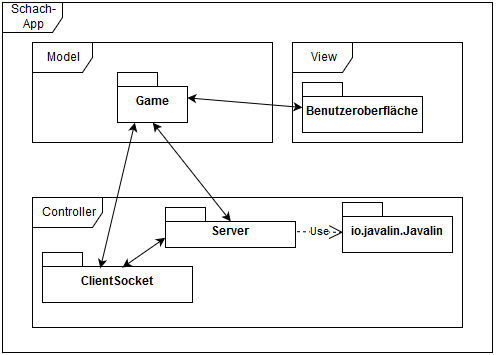
\includegraphics[width=1\linewidth]{Diagramme/Paketdiagramm}
			\captionof{figure}{Paketdiagramm}
			\label{fig:Paketdiagramm}
		\end{minipage}
		\subsection{\gls{GUI}}
		
		\subsection{Server}
		Der Server wurde nach dem \gls{REST} Prinzip entworfen. Alle Anfragen werden per \gls{URL} gesendet. Benachrichtigungen über neue Züge erfolgen über eine \gls{WS}-Verbindung. Da Züge abwechselnd und meist nicht direkt nacheinander ausgeführt werden, wurde sich gegen eine konstante Verbindung zum Zugaustausch entschieden.
		
		\subsection{Spiellogik}
		Die Spiellogik wird komplett selbst implementiert ohne externe Bibliotheken zu benutzen. Zur Spielmodellierung werden verschiedene Konzepte als Klassen implementiert. Die Spiellogik muss zum einen über einen Zug/Brettverwalter mit der Benutzeroberfläche kommunizieren können, um das Spiel in Echtzeit visualisieren zu können, als auch dem Server zur Verfügung stehen, damit dieser die Spielregeln überwachen und über den Spielzustand Bescheid wissen kann.
	\section{Klassendiagramme}
	
		\subsection{Spiel}
		
		\begin{minipage}{\linewidth}
			\centering
			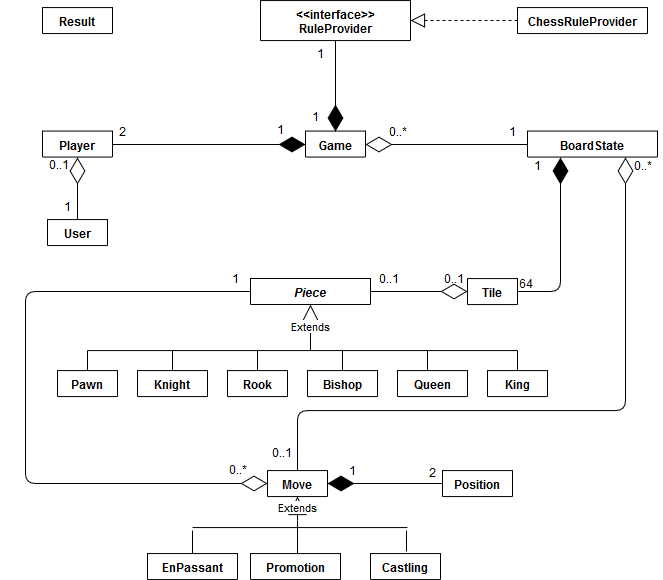
\includegraphics[width=1\linewidth]{Diagramme/TotalGame}
			\captionof{figure}{TotalGame}
			\label{fig:Spiellogik}
		\end{minipage}
		\newpage
		\textbf{\Large{Spiel}}
				\begin{description}
					\item \textbf{Game} stellt ein Spiel dar. Es besteht aus zwei Spielern \textbf{Player} und einem Spielfeld \textbf{BoardState}. Außerdem benutzt es eine Instanziierung des Interface \textbf{RuleProvider}, welches die Regeln für ein beliebiges Spiel auf einem Schachbrett liefert. Die Regeln samt Startkonfiguration des Brettes auf ein Interface auszulagern anstatt sie ins \textbf{Game} direkt einzubauen macht die Spiellogik leichter austauschbar und ermöglicht zum Beispiel das Erstellen weiterer Spielvarianten. Diese könnten dann einfach in dem Konsturktor der \textbf{Game} Klasse mitgegeben werden. Auch könnte man so beispielsweise einen Spieler mit einem einstellbaren Figurendefizit in das Spiel startet lassen, indem man einen \textbf{RuleProvider} mit entsprechender Anfangsstellung einfügt.
					\item In unserem Fall wird das Interface nur von der Klasse \textbf{ChessRuleProvider} implementiert, welche die Standard-Schachregeln liefert. Diese Klasse hat bei einer Methode als Rückgabewert ein Objekt vom Typ \textbf{Result}. Ergebnisse als eigenes Objekt zu behandeln anstatt diese einfach nur als String anzugeben hat den Vorteil, dass zum Ergebnis an sich auch eine Begründung mitgeliefert werden kann, welche der Spieler nach Spielende einsehen kann. Außerdem ist ein Ergebnis so auch immer als ein solches erkennbar.
					\item Ein \textbf{Player} ist ein Spieler eines konkretes Spiels und besteht aus einem \textbf{User}, welcher einen Benutzer im Allgemeinen darstellt. Umgekehrt muss ein \textbf{User} aber nicht zu jedem Zeitpunkt einen \textbf{Player} haben. Das Trennen der Konzepte Spieler und Benutzer ermöglicht das Hinzufügen von Spielern zu bestimmten \textbf{Game}-Objekten, ohne Benutzer direkt an ein Spiel koppeln zu müssen.
					\item Das Spielfeld \textbf{BoardState} enthält 64  \textbf{Tiles} (Schachfelder) und einen \textbf{Move}, welcher hier den letzten ausgeführten Zug des Spiels darstellt. Das Speichern des zuletzt ausgeführten Zuges ist für den Zug \glqq en passant\grqq\ sowie zur Überprüfung gespielter Züge bei Übertragung des Brettes notwendig.
					\item Ein \textbf{Tile} kann ein \textbf{Piece} enthalten, muss es aber nicht. Das Brett als Array von \textbf{Tiles} mit Figuren zu speichern ist notwendig, um zu jedem Zeitpunkt jedes Feld zur Hand zu haben und auf dieses Figuren setzen und entfernen zu können. Leere Felder können einfach erkannt werden, nämlich wenn sie kein Objekt vom Typ Piece enthalten.
					\item \textbf{Piece} ist eine abstrakte Klasse und stellt eine Figur dar. Sie wird von den sechs konkreten Figurenklassen beerbt. Diese speichern Informationen über ihren Wert, ihre Darstellung als Zeichen sowie ihre Zugfähigkeiten. Dadurch werden switch-case Abfragen vermieden, und von jeder Figur kann direkt der gewünschte Wert/das Verhalten angefordert werden, ohne über den Typ Bescheid wissen zu müssen.
					\item Ein \textbf{Move} besteht im Allgemeinen nur aus zwei \textbf{Positionen}. Ein Zug muss über die ziehende Figur nicht Bescheid wissen, da zur Ausführung des Zuges ohnehin das gesamte Brett mit allen Positionen aller Figuren vorliegen muss. Es gibt drei Spezialfälle eines Zuges, welche eine gesonderte Implementierung benötigen, da sie neben zwei Positionen noch andere Informationen enthalten müssen. Diese erben alle von \textbf{Move}, da diese trotzdem aus einer Start- und Zielposition bestehen. Das macht das Erstellen und Weitergeben von Listen von Zügen einfacher, und ermöglicht eine einfache Ausführung auf der Benutzeroberfläche.
					\item \textbf{Position} stellt eine Position auf einem Schachbrett dar und besteht aus zwei Zahlen, welche die Koordinaten darstellen. Diese müssen zwischen 0-7 liegen, was beim Erstellen eines solchen Objektes sichergestellt wird. Das hat den Vorteil, dass Positionen nicht bei jeder Nutzung auf Korrektheit überprüft werden müssen um Programmabstürze zu vermeiden.
				\end{description}		
		\newpage
		
		\subsubsection{Game}
		\begin{minipage}{\linewidth}
			\centering
			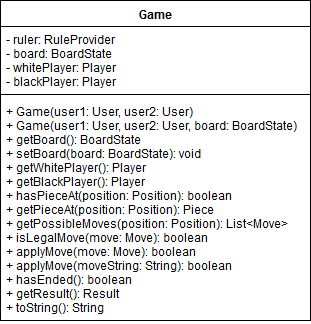
\includegraphics[width=1\linewidth]{Diagramme/Game}
			\captionof{figure}{Game}
			\label{fig:game}
		\end{minipage}
		
			\textbf{\Large{Game:}}
			
			Stellt ein Spiel dar, verwaltet teilnehmende Spieler, Regelwerk sowie Brettzustand. \\
				\\
				\textbf{\large{Attribute}}
				\newline
				\rule{\textwidth}{1pt}
				
				\begin{description}
					 \item \textbf{- ruler: RuleProvider}\\ Objekt, welches das Interface RuleProvider implementiert und die Spielregeln zur Verfügung stellt.
					 \item \textbf{- board: BoardState}\\ Hier wird der aktuelle Spielstatus bestehend aus
					 \begin{itemize}
					 
			\item Stand aller Figuren auf dem Brett
			\item mögliche Rochaden
			\item letzter ausgeführter Spielzug
			\item Anzahl der Züge ohne Bauernzug oder Schlagen von Figuren
			  \end{itemize}	
			  	 gespeichert.
					 \item \textbf{- whitePlayer: Player}\\ Der Spieler mit den weißen Figuren.
					 \item \textbf{- blackPlayer: Player}\\ Der Spieler mit den schwarzen Figuren.\\
			    \\
				\end{description} 
				
				 \textbf{\large{Methoden}}
				 \newline
		 		\rule{\textwidth}{1pt}
	 			\begin{description}
					 \item \textbf{+ Game(user1: User ,user2: User)}\\ Konstruktor, welcher ein Spiel mit den Standard Schachregeln und einem Brett auf Anfangsposition erzeugt. Der zuerst übergebene User erhält die weißen Figuren, der zweite die schwarzen.
					 \item \textbf{+ Game(user1: User ,user2: User, board: BoardState)}\\ Konstruktor, welcher ein Spiel mit den Standard Schachregeln und dem übergebenen Brettstatus erzeugt. Der zuerst übergebene \textbf{User} erhält die weißen Figuren, der zweite die schwarzen.
					 \item \textbf{+ getBoard(): BoardState}\\ Gibt den Brettstatus \textbf{board}des akutellen Spiels zurück.
					\item \textbf{+ getBoard(board: BoardState): void}\\ Setzt den Brettstatus \textbf{board} auf das übergebene Objekt.
					\item \textbf{+ getWhitePlayer(): Player}\\ Gibt den weißen Spieler \textbf{whitePlayer} zurück.
					\item \textbf{+ getBlackPlayer(): Player}\\ Gibt den schwarzen Spieler \textbf{blackPlayer} zurück.
					\item \textbf{+ hasPieceAt(position: Position): boolean} Gibt zurück, ob sich an der übergebenen Position auf dem Brett eine Figur befindet.
					\item \textbf{+ getPieceAt(position: Position): Piece}\\ Gibt die Figur zurück, welche sich an der übergebZüge Position befindet. Ist die Position nicht dibesetz wird \textbf{null} zurückgegeben.        ausführ     item \textbf{+ getPossiblePositions(position: Position): List<Position>}\\ Gibt alle möglichen Positionen als Liste zurück, auf welche eine Figur, welche sich auf der übergebenen Position befindet, ziehen kann. Zum Berechnen dieser wird das \textbf{ruler} Objekt benutzt.
					\item \textbf{+ applyMove(move: Move): void}\\ Führt den übergebenen Zug auf dem Spielbrett \textbf{board} aus.
					\item \textbf{+ applyMove(moveString: String): void}\\ Führt den als String übergebenen Zug auf dem Spielbrett \textbf{board} aus. Dazu muss der String erst in ein Objekt vom Typ \textbf{Move} umgewandelt werden.
					\item \textbf{+ hasEnded(): boolean}\\ Gibt zurück, ob das Spiel gemäß den Schachregeln beendet ist. Dazu wird das \textbf{ruler} Objekt benutzt.
					\item \textbf{+ getResult(): Result}\\ Gibt das Ergebnis eines Spiels als Objekt vom Typ \textbf{Result} zurück. Ist das Spiel noch nicht beendet, wird \textbf{null} zurückgegeben.
					\item \textbf{+ toString(): String}\\ Wandelt den gesamten Spielstatus in eine Zeichenkette um. Dazu werden die Benutzernamen sowie die String-Repräsentation des \textbf{board} Objekts genutzt.
				\end{description}
			
			
		\newpage
		
		\subsubsection{RuleProvider}
		\begin{minipage}{\linewidth}
			\centering
			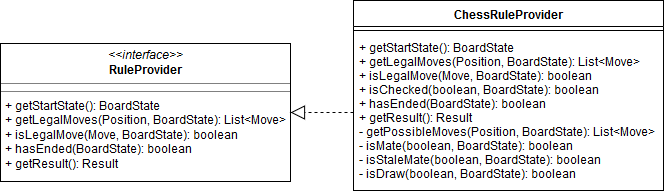
\includegraphics[width=1\linewidth]{Diagramme/RuleProvider}
			\captionof{figure}{RuleProvider}
			\label{fig:ruleProvider}
		\end{minipage}
		\begin{itemize}
			\item \textbf{\Large{RuleProvider}}
			
			Interface, welches alle nötigen Regeln eines Spiels auf einem Schachbrett bereitstellt.\\
			\\			
				\textbf{\large{Methoden}}
				\newline
				\rule{\textwidth}{1pt}
				\begin{description}			
					\item \textbf{+ getStartState(): BoardState}\\ Soll die Anfangskonfiguration eines Brettes für das jeweilige Spiel zurückgeben.
					\item \textbf{+ getLegalMoves(position: Position, board: BoardState): List<Move>}\\ Soll auf einem Brett ausgehend von einer Position die Zugmöglichkeiten der sich darauf befindenden Figur berechnen, entsprechend der implementierten Regeln.
					\item \textbf{+ isLegalMove(move: Move, board: BoardState): boolean}\\ Soll überprüfen, ob ein Zug gemäß der jeweiligen Regeln auf einem bestimmten Brett erlaubt ist.
					\item \textbf{+ hasEnded(board: BoardState): boolean}\\ Soll prüfen, ob das Spiel auf einem bestimmten Brett gemäß den jeweiligen Regeln beendet ist.
					\item \textbf{+ getResult(board: BoardState): Result}\\ Soll das Ergebnis eines Spiels als \textbf{Result} zurückgeben. Ist das Spiel nicht beendet soll \textbf{null} zurückgegeben werden.\\
				\\
				\end{description}
			
			\item \textbf{\Large{ChessRuleProvider}} 
					
			Konkreter Regellieferer, welcher die genauen Schachregeln zur Verfügung stellt.\\
				\\
				\textbf{\large{Methoden}}
				\newline
				\rule{\textwidth}{1pt}
				\begin{description}
					\item \textbf{+ getStartState(): BoardState}\\ Gibt die Standard Anfangsstellung eines Schachspiels als \textbf{BoardState} zurück.
					\item \textbf{+ getLegalMoves(position: Position, board: BoardState): List<Move>}\\ Gibt eine Liste an erlaubten Zügen ausgehend von einer ausgewählten Position und einem Brett zurück. Dazu werden zunächst mit \textbf{getPossibleMoves(Position, BoardState)} alle möglichen Züge berechnet. Anschließen wird jeder Zug auf einer Kopie des Brettes simuliert, und mithilfe von \textbf{isChecked(boolean, BoardState)} überprüft, ob der selbe Spieler danach im Schach stünde (was den Zug ungültig machen würde).
					\item \textbf{+ isLegalMove(move: Move, board: BoardState): boolean}\\ Prüft, ob ein Zug gemäß den Schachregeln auf dem übergebenen Brett erlaubt ist.
					\item \textbf{+ isChecked(white: boolean, board: BoardState): boolean}\\ Überprüft ob ein Spieler auf dem gegebenen Brett im Schach steht. Ist der übergebene boolean true, wird Weiß überprüft, bei false Schwarz. Dazu wird geschaut, ob es eine gegnerische Figur gibt, welche durch \textbf{getPosssibleMoves(Position, BoardState)} einen Zug erhält, mit welchem der eigene König erreicht werden könnte.
					\item \textbf{+ hasEnded(board: BoardState): boolean}\\ Prüft, ob das Schachspiel zu Ende ist. Dazu wird geprüft, ob der zu ziehende Spieler laut \textbf{isMate(BoardState)} Matt gesetzt, laut \textbf{isStaleMate(BoardState)} Patt gesetzt oder ob laut  \textbf{isDraw(BoardState)} andersweitig ein Unentschieden erreicht wurde.
					\item \textbf{+ getResult(): Result}\\ Ruft \textbf{hasEnded(BoardState board)} auf, gibt aber bei beendetem Spiel das jeweilige Ergebnis als \textbf{Result} zurück. Ist das Spiel nicht beendet wird \textbf{null} zurückgegeben.
					\item \textbf{- getPossibleMoves(position: Position, board: BoardState): List<Move>}\\ Gibt alle möglichen Züge einer Figur auf dem Brett zurück, ohne dabei zu berücksichtigen, ob der ziehende Spieler nach diesem Zug im Schach stehen würde. Dazu wird die jeweilige \textbf{getMovement()}-Methode der Figur an der angegebenen Position ausgeführt.				
					\item \textbf{- isMate(board: BoardState): boolean}\\ Prüft, ob der zu ziehende Spieler Matt gesetzt wurde. Das ist der Fall, wenn der Spieler laut \textbf{isChecked(boolean, BoardState)} im Schach steht, und es für keine Figur einen nach \textbf{getLegalMoves(Position, BoardState)}erlaubten Zug gibt.
					\item \textbf{- isStaleMate(board: BoardState): boolean}\\ Prüft, ob der zu ziehende Spieler Patt gesetzt wurde. Das ist der Fall, wenn der Spieler laut \textbf{isChecked(boolean, BoardState)} nicht im Schach steht, und es für keine Figur einen nach \textbf{getLegalMoves(Position, BoardState)}erlaubten Zug gibt.
					\item \textbf{- isDraw(board: BoardState): boolean}\\ Prüft, ob ein anderweitiges Unentschieden erreicht wurde. Dies ist der Fall, wenn zu wenig Figuren auf dem Brett vorhanden sind um Matt zu setzen, oder wenn 50 Züge lang keine Figur geschlagen und kein Bauer gezogen wurde, also wenn der \textbf{movesWithoutAction}-Wert des \textbf{board}-Objekts 50 (oder größer) ist.
				\end{description}
		\end{itemize}
		\newpage
		\subsubsection{BoardState}
		\begin{minipage}{\linewidth}
			\centering
			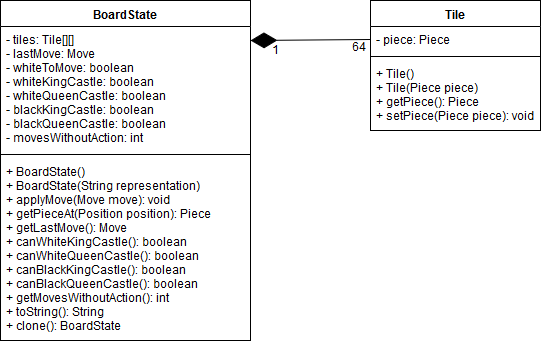
\includegraphics[width=1\linewidth]{Diagramme/BoardState}
			\captionof{figure}{BoardState}
			\label{fig:boardState}
		\end{minipage}
	
		\begin{itemize}
			\item \textbf{\Large{BoardState}}	
			
			Der gesamte Status eines Schachspiels der notwendig ist, um ein Spiel rekonstruieren und alle Regeln überprüfen zu können.\\
			\\
				\textbf{\large{Attribute}}
				\newline
				\rule{\textwidth}{1pt}
			
				\begin{description}				
					\item \textbf{- tiles: Tile[][]}\\ Ein Array von Tiles, welches den Aufbau des Spielbretts darstellt
					 \item \textbf{- lastMove: Move}\\ Der letzte gespielte Zug.
					 \item \textbf{- whiteToMove: boolean}\\ Speichert, ob Weiß am Zug ist.
					 \item \textbf{- whiteKingCastle: boolean}\\ Speichert ab, ob Weiß noch auf der Königsseite rochieren kann.
					 \item \textbf{- whiteQueenCastle: boolean}\\ Speichert ab, ob Weiß noch auf der Damenseite rochieren kann.
					 \item \textbf{- blackKingCastle: boolean}\\ Speichert ab, ob Schwarz noch auf der Königsseite rochieren kann.
					 \item \textbf{- blackQueenCastle: boolean}\\ Speichert ab, ob Schwarz noch auf der Damenseite rochieren kann.
					\item \textbf{- movesWithoutAction: int}\\ Speichert die Anzahl der Züge in Folge, in welcher kein Bauer gezogen und keine Figur geschlagen wurde.\\
				\\
				\end{description}
				\textbf{\large{Methoden}}
				\newline
				\rule{\textwidth}{1pt}
				\begin{description}
					\item \textbf{+ BoardState()}\\ Erzeugt ein leeres Schachbrett und setzt alle Variablen auf ihre Standardwerte.
					\item \textbf{+ BoardState(representation: String)} Erzeugt ein Brett, ausgehen von einem String. In diesem müssen alle notwendigen Informationen in einem einheitlichen Format gespeichert sein.
					\item \textbf{+ applyMove(move: Move): void}\\ Führt einen Zug auf dem Brett aus, indem es die Figur(en) wie im Move-Objekt vorgegeben bewegt und möglicherweise andere Figuren schlägt(überschreibt). Außerdem wird die zu ziehende Farbe, der letzte Zug, sowie die Anzahl der Züge ohne Aktion aktualisiert. Bei entsprechender Verletzung werden möglich Rochaden auf \textbf{false} gesetzt.
					\item \textbf{+ getPieceAt(position: Position): Piece}\\ Gibt die Figur an der übergebenen Position zurück. Ist die Position nicht besetzt, wird \textbf{null} zurückgegeben.			
					\item \textbf{+ getLastMove(): Move}\\ Gibt \textbf{lastMove} zurück.
					 \item \textbf{+ canWhiteKingCastle(): boolean}\\ Gibt zurück, ob Weiß noch auf der Königsseite rochieren kann.
					 \item \textbf{+ canWhiteQueenCastle(): boolean}\\ Gibt zurück, ob Weiß noch auf der Damenseite rochieren kann.
					 \item \textbf{+ canBlackKingCastle(): boolean}\\ Gibt zurück, ob Schwarz noch auf der Königsseite rochieren kann.
					 \item \textbf{+ canBlackQueenCastle(): boolean}\\ Gibt zurück, ob Schwarz noch auf der Damenseite rochieren kann.
					 \item \textbf{+ getMovesWithoutAction): int}\\ Gibt \textbf{movesWithoutAction} zurück.
					 \item \textbf{+ toString(): String}\\ Gibt den gesamten Brettzustand als String codiert zurück. Aus diesem String muss mithilfe des entsprechenden Konstruktors ein identisches Brett erzeugt werden können.		
					 \item \textbf{+ clone(): BoardState}\\ Erzeugt und übergibt ein identisches Spielbrett, indem die String-Repräsentation des aktuellen Brettes als Parameter des Konstruktors verwendet wird.	\\						\\
				\end{description}
			
			\item \textbf{\Large{Tile}}
			
			Stellt eine Feld eines Schachbretts dar.\\
			\\
				\textbf{\large{Attribute}}
				\newline
				\rule{\textwidth}{1pt}
			
				\begin{description}					
					\item \textbf{- piece: Piece}\\ Die Figur, welche sich auf dem Feld befindet. Befindet sich keine Figur auf dem Feld, steht hier \textbf{null}.\\
					\\
				\end{description}
				\textbf{\large{Methoden}}
				\newline
				\rule{\textwidth}{1pt}
				\begin{description}
					\item \textbf{+ Tile()}\\ Konstruktor, welcher ein leeres Feld erzeugt.
					\item \textbf{+ Tile(piece: Piece)}\\ Konstruktor, welcher ein Feld mit der übergebenen Figur darauf erzeugt.
					\item \textbf{+ getPiece(): Piece}\\ Gibt \textbf{piece} zurück. Wurde kein \textbf{Piece} gesetzt, wird \textbf{null} zurückgegeben.
					\item \textbf{+ setPiece(piece: Piece): void}\\ Setzt \textbf{piece} auf die übergebene Figur.
				\end{description}
			
		\end{itemize}
		\newpage		
		
		\subsubsection{Player}
		\begin{minipage}{\linewidth}
			\centering
			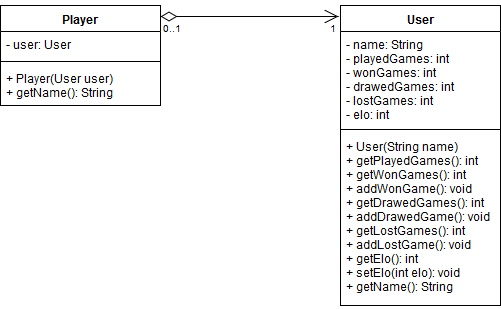
\includegraphics[width=1\linewidth]{Diagramme/Player}
			\captionof{figure}{Player}
			\label{fig:player}
		\end{minipage}
		\begin{itemize}
			\item \textbf{\Large{Player}}
			
			Stellt einen Spieler eines konkretes Spiels dar. Existiert nur während das jeweilige Spiel existiert.\\
			\\
				\textbf{\large{Attribute}}
				\newline
				\rule{\textwidth}{1pt}
				
				\begin{description}					
					\item \textbf{- user: User}\\ Der mit diesem Spielerobjekt verknüpfte Benutzer.\\
					\\
				\end{description}
				\textbf{\large{Methoden}}
				\newline
				\rule{\textwidth}{1pt}
				\begin{description}
					\item \textbf{+ Player(user: User)}\\ Konstruktor, welcher \textbf{user} auf den übergebenen \textbf{User} setzt.
					\item \textbf{+ getName(): String}\\ Gibt den Namen des verknüpften Benutzers als String zurück.\\
				\\
				\end{description}
			
			\item \textbf{\Large{User}}
			
			Stellt einen Benutzer der Schach-App dar. \\
			\\
				\textbf{\large{Attribute}}
				\newline
				\rule{\textwidth}{1pt}
				
				\begin{description}
					\item \textbf{- name: String}\\ Der eindeutige Name eines Benutzers.
					\item \textbf{- playedGames: int}\\ Die Anzahl der gespielten Spiele des Benutzers.
					\item \textbf{- wonGames: int}\\ Die Anzahl der gewonnenen Spiele des Benutzers.
					\item \textbf{- drawedGames: int}\\ Die Anzahl der remisierten Spiele des Benutzers.
					\item \textbf{- lostGames: int}\\ Die Anzahl der verlorenen Spiele des Benutzers.
					\item \textbf{- elo: int}\\ Der Elo-Wert des Benutzers.\\
				\\
				\end{description}
				\textbf{\large{Methoden}}
				\newline
				\rule{\textwidth}{1pt}
				\begin{description}
					\item \textbf{+ User(name: String)}\\ Erstellt einen neuen Benutzer mit dem übergebenen Namen. Setzt \textbf{elo} auf 1000, alle anderen Attribute auf 0. 
					\item \textbf{+ getPlayedGames(): int}\\ Gibt \textbf{playedGames} zurück.
					\item \textbf{+ getWonGames(): int}\\ Gibt \textbf{wonGames} zurück.
					\item \textbf{+ addWonGame(): void}\\ Erhöht \textbf{wonGames} und \textbf{playedGames} um eins.
					\item \textbf{+ getDrawedGames(): int}\\ Gibt \textbf{drawedGames} zurück.
					\item \textbf{+ addDrawedGame(): void}\\ Erhöht \textbf{drawedGames} und \textbf{playedGames} um eins.
					\item \textbf{+ getLostGames(): int}\\ Gibt \textbf{lostGames} zurück.				
					\item \textbf{+ addLostGame(): void}\\ Erhöht \textbf{lostGames} und \textbf{playedGames} um eins.
					\item \textbf{+ getElo(): int}\\ Gibt \textbf{elo} zurück.
					\item \textbf{+ setElo(Elo: int): void}\\ Setzt die Elo des Benutzers auf den übergebenen Wert.
					\item \textbf{+ getName(): String}\\ Gibt \textbf{name} zurück.					
				\end{description}
		\end{itemize}
		\newpage	
			
		\subsubsection{Result}
		
		\begin{minipage}{\linewidth}
			\centering
			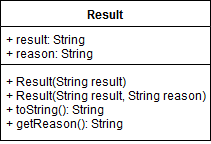
\includegraphics[width=1\linewidth]{Diagramme/Result}
			\captionof{figure}{Result}
			\label{fig:result}
		\end{minipage}
		\textbf{\Large{Result}}
			
			Stellt ein Ergebnis eines Spiels dar.\\
			\\
				\textbf{\large{Attribute}}
				\newline
				\rule{\textwidth}{1pt}
			
				\begin{description}					
					\item \textbf{- result: String}\\ Das Ergebnis eines Spiels als String codiert.
					\item \textbf{- reason: String}\\ Eine optionale Begründung zum Ergebnis als String.\\
					\\
				\end{description}
				\textbf{\large{Methoden}}
				\newline
				\rule{\textwidth}{1pt}
				\begin{description}
					\item \textbf{+ Result(result: String)}\\ Erzeugt ein Objekt mit dem übergebenen String als \textbf{result} und einer leeren \textbf{reason}.
					\item \textbf{+ Result(result: String, reason: String)}\\ Erzeugt ein Objekt mit dem ersten übergebenen String als \textbf{result} und dem zweiten übergebenen String als \textbf{reason}.
					\item \textbf{+ toString(): String}\\ Gibt \textbf{result} zurück.
					\item \textbf{+ getReson(): String} Gibt \textbf{reason} zurück.						
				\end{description}		
		\newpage
		
		\subsubsection{Move}
		
		\begin{minipage}{\linewidth}
			\centering
			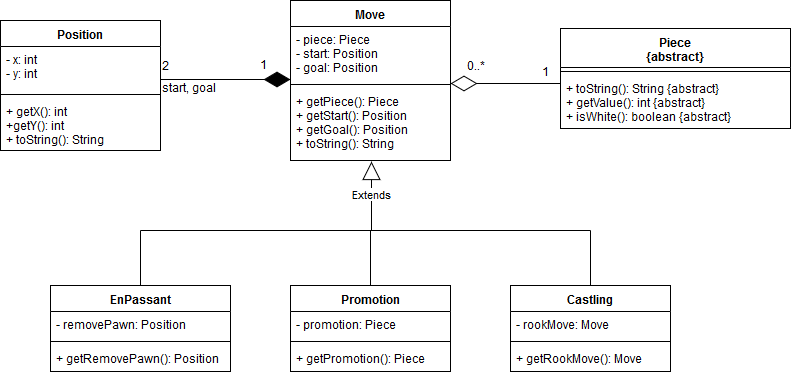
\includegraphics[width=1\linewidth]{Diagramme/Move}
			\captionof{figure}{Move}
			\label{fig:move}
		\end{minipage}
		\begin{itemize}
			\item \textbf{\Large{Move}}
			
			Stellt einen Zug dar, ohne über die zu ziehende Figur Bescheid zu wissen.\\
			\\
				\textbf{\large{Attribute}}
				\newline
				\rule{\textwidth}{1pt}
			
				\begin{description}				
					\item \textbf{- start: Position}\\ Position, von welcher aus der Zug ausgeführt wird.
					\item \textbf{- goal: Position}\\ Position, zu welcher der Zug hinführt.\\
					\\
				\end{description}
				\textbf{\large{Methoden}}
				\newline
				\rule{\textwidth}{1pt}
				\begin{description}
					\item \textbf{+ Move(start: Position, goal: Position)}\\ Erzeugt einen Zug mit der übergebenen Start- und Zielposition.				
					\item \textbf{+ getStart(): Position}\\ Gibt \textbf{start} zurück.
					\item \textbf{+ getGoal(): Position}\\ Gibt \textbf{goal} zurück.
					\item \textbf{+ toString(): String}\\ Gibt eine eindeutige Repräsentation des Zugs als Zeichenkette zurück.
				\end{description}
			
			\item \textbf{\Large{Position}}
			
			Stellt eine Position auf einem Schachbrett dar.\\
			\\
				\textbf{\large{Attribute}}
				\newline
				\rule{\textwidth}{1pt}
			
				\begin{description}			
					\item \textbf{- x: int}\\ Stellt die horizontale Koordinate auf dem Schachbrett dar.,
					\item \textbf{- y: int}\\ Stellt die vertikale Koordinate auf dem Schachbrett dar.\\
					\\
				\end{description}
				\textbf{\large{Methoden}}
				\newline
				\rule{\textwidth}{1pt}
				\begin{description}
					\item \textbf{+ Position(x: int, y: int)}\\ Erzeugt eine Position mit den angegebenen Koordinaten. Liegen die Koordinaten außerhalb eines Schachbretts wird eine Exception ausgelöst.
					\item \textbf{+ Position(representation: String)}\\ Erzeugt eine Position indem der übergebene String in Koordinaten umgewandelt wird. Liegen die Koordinaten außerhalb eines Schachbretts wird eine Exception ausgelöst.
					\item \textbf{+ getX(): int}\\ Gibt \textbf{\textit{x}} zurück.
					\item \textbf{+ getY(): int}\\ Gibt \textbf{\textit{y}} zurück.
					\item \textbf{+ toString(): String}\\ Gibt eine Repräsentation der Position als String zurück.\\
					\\
				\end{description}
			
			\item \textbf{\Large{EnPassant}}
			
			Stellt den Bauernzug en passant dar.\\
			\\
				\textbf{\large{Attribute}}
				\newline
				\rule{\textwidth}{1pt}
			
				\begin{description}
					\item \textbf{- removePawn: Piece}\\ Die Position des Bauern, der mit diesem Zug geschlagen wird.\\
					\\
				\end{description}
				\textbf{\large{Methoden}}
				\newline
				\rule{\textwidth}{1pt}
				\begin{description}
					\item \textbf{+ EnPassant(start: Position, goal: Position)}\\ Ruft den Konstruktor von \textbf{Move} auf, berechnet und setzt die Position\textbf{removePawn}.
					\item \textbf{+ getRemovePawn(): Position}\\ Gibt \textbf{removePawn} zurück.
					\item \textbf{+ toString(): String}\\ Gibt eine eindeutige Repräsentation des Zugs als Zeichenkette zurück.\\
					\\
				\end{description}	
			
			\item \textbf{\Large{Promotion}}
			
			Stellt eine Bauernumwandlung dar.\\
			\\
				\textbf{\large{Attribute}}
				\newline
				\rule{\textwidth}{1pt}
				\begin{description}				
					\item \textbf{- promotion: Piece}\\ Die Figur, in welche sich der Bauer verwandeln soll.\\
					\\
				\end{description}
				\textbf{\large{Methoden}}
				\newline
				\rule{\textwidth}{1pt}
				\begin{description}
					\item \textbf{+ Promotion(start: Position, goal: Position, promo: Piece)}\\ Ruft den Konstruktor von \textbf{Move} auf und setzt \textbf{promotion} auf die übergebene Figur.
					\item \textbf{+ getPromotion(): Piece}\\ Gibt \textbf{promotion} zurück.
					\item \textbf{+ toString(): String}\\ Gibt eine eindeutige Repräsentation des Zugs als Zeichenkette zurück.\\
					\\
				\end{description}
			
			\item \textbf{\Large{Castling}}
			
			Stellt eine Rochade dar.\\
			\\
				\textbf{\large{Attribute}}
				\newline
				\rule{\textwidth}{1pt}
			
				\begin{description}				
					\item \textbf{- rookMove: Move}\\ Die Bewegung des Turms, welche zusätzlich zu der des Königs mit diesem Zug ausgeführt wird.\\
					\\
				\end{description}
				\textbf{\large{Methoden}}
				\newline
				\rule{\textwidth}{1pt}
				\begin{description}
					\item \textbf{+ Castling(start: Position, goal: Position)}\\ Ruft den Konstruktor von \textbf{Move} auf, berechnet und setzt den Zug\textbf{rookMove}.
					\item \textbf{+ getRookMove(): Move}\\ Gibt \textbf{rookMove} zurück.
					\item \textbf{+ toString(): String}\\ Gibt eine eindeutige Repräsentation des Zugs als Zeichenkette zurück.
				\end{description}			
		\end{itemize}
		\newpage
		
		\subsubsection{Pieces}
		
		\begin{minipage}{\linewidth}
		\centering
		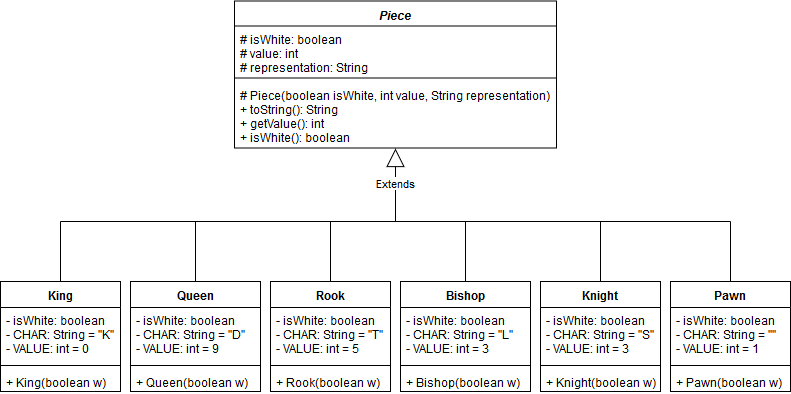
\includegraphics[width=1\linewidth]{Diagramme/Pieces}
		\captionof{figure}{Pieces}
		\label{fig:pieces}
		\end{minipage}
		\begin{itemize}
			\item \textbf{\Large{Piece}}
			
				Stellt das abstrakte Konzept einer Schachfigur dar.\\
				\\				
				\textbf{\large{Attribute}}
				\newline
				\rule{\textwidth}{1pt}
				\begin{description}			
					\item \textbf{- isWhite: boolean}\\ Speichert, ob die Figur weiß ist.
					\item \textbf{- value: int}\\ Speichert den Wert einer Figur ab.
					\item \textbf{- representation: String}\\ Speichert das repräsentative Zeichen einer Figur ab.\\
					\\
				\end{description}
				\textbf{\large{Methoden}}
				\newline
				\rule{\textwidth}{1pt}
				\begin{description}
					\item \textbf{+ Piece(isWhite: boolean, value: int, representation: String)}\\ Erzeugt eine neue Figur, setzt alle Attribute auf die jeweiligen übergebenen Werte.
					\item \textbf{+ toString(): String}\\ Gibt \textbf{representation} zurück.
					\item \textbf{+ getValue(): int}\\ Gibt \textbf{value} zurück.
					\item \textbf{+ isWhite(): boolean}\\ Gibt \textbf{isWhite} zurück.				
				\end{description}
			
			\item \textbf{\Large{King}}
			
				Stellt einen König dar.\\
				\\				
				\textbf{\large{Attribute}}
				\newline
				\rule{\textwidth}{1pt}
				\begin{description}			
					\item \textbf{- CHAR: String}\\ Die Repräsentation eines Königs, wird auf \glqq K\grqq\  gesetzt.
					\item \textbf{- VALUE: int}\\ Der Wert eines Königs, wird auf 0 gesetzt, da dem König an sich kein Wert zugewiesen werden kann.\\
					\\
				\end{description}
				\textbf{\large{Methoden}}
				\newline
				\rule{\textwidth}{1pt}
				\begin{description}
					\item \textbf{+ King(w: boolean)}\\ Erzeugt einen neuen König. Dazu wird der Konstruktor von \textbf{Piece} aufgerufen, als Parameter werden w, \textbf{VALUE}, und \textbf{CHAR} übergeben.
					\item \textbf{+ getMovement(p: Position, b: BoardState): List<Move>}\\ Gibt eine Liste der Züge zurück, die ein König auf dem gegebenen Schachbrett von der gegebenen Position aus ausführen kann, inklusive Rochade. Dabei wird nicht berücksichtigt, ob sich der König nach dem Zug in Schach befinden würde.\\
					\\
				\end{description}
				
			
			\item \textbf{\Large{Queen}}
			
				Stellt eine Dame dar.\\
				\\				
				\textbf{\large{Attribute}}
				\newline
				\rule{\textwidth}{1pt}
				\begin{description}				
					\item \textbf{- CHAR: String}\\ Die Repräsentation einer Dame, wird auf \glqq D\grqq\ gesetzt.
					\item \textbf{- VALUE: int}\\ Der Wert einer Dame, wird auf 9 gesetzt.\\
					\\
				\end{description}
				\textbf{\large{Methoden}}
				\newline
				\rule{\textwidth}{1pt}
				\begin{description}	
					\item \textbf{+ Queen(w: boolean)}\\ Erzeugt eine neue Dame. Dazu wird der Konstruktor von \textbf{Piece} aufgerufen, als Parameter werden w, \textbf{VALUE}, und \textbf{CHAR} übergeben.
					\item \textbf{+ getMovement(p: Position, b: BoardState): List<Move>}\\ Gibt eine Liste der Züge zurück, die eine Dame auf dem gegebenen Schachbrett von der gegebenen Position aus ausführen kann. Dabei wird nicht berücksichtigt, ob sich der König des ziehenden Spielers nach dem Zug in Schach befinden würde.\\
					\\
				\end{description}
			
			\item \textbf{\Large{Rook}}
				
				Stellt einen Turm dar.\\
				\\				
				\textbf{\large{Attribute}}
				\newline
				\rule{\textwidth}{1pt}
				\begin{description}
					\item \textbf{- CHAR: String}\\ Die Repräsentation eines Turms, wird auf \glqq T\grqq\ gesetzt.
					\item \textbf{- VALUE: int}\\ Der Wert eines Turms, wird auf 5 gesetzt.\\
					\\
				\end{description}
				\textbf{\large{Methoden}}
				\newline
				\rule{\textwidth}{1pt}
				\begin{description}	
					\item \textbf{+ Rook(w: boolean)}\\ Erzeugt einen neuen Turm. Dazu wird der Konstruktor von \textbf{Piece} aufgerufen, als Parameter werden w, \textbf{VALUE}, und \textbf{CHAR} übergeben.
					\item \textbf{+ getMovement(p: Position, b: BoardState)}\\ Gibt eine Liste der Züge zurück, die ein Turm auf dem gegebenen Schachbrett von der gegebenen Position aus ausführen kann. Dabei wird nicht berücksichtigt, ob sich der König des ziehenden Spielers nach dem Zug in Schach befinden würde.\\
					\\
				\end{description}
			
			\item \textbf{\Large{Bishop}}
				
				Stellt einen Läufer dar.\\
				\\
				\textbf{\large{Attribute}}
				\newline
				\rule{\textwidth}{1pt}
				\begin{description}			
					\item \textbf{- CHAR: String}\\ Die Repräsentation eines Läufers, wird auf \glqq L\grqq\ gesetzt.
					\item \textbf{- VALUE: int}\\ Der Wert eines Läufers, wird auf 3 gesetzt.\\
					\\
				\end{description}
				\textbf{\large{Methoden}}
				\newline
				\rule{\textwidth}{1pt}	
				\begin{description}				
					\item \textbf{+ Bishop(w: boolean)}\\ Erzeugt einen neuen Läufer. Dazu wird der Konstruktor von \textbf{Piece} aufgerufen, als Parameter werden w, \textbf{VALUE}, und \textbf{CHAR} übergeben.
					\item \textbf{+ getMovement(p: Position, b: BoardState)}\\ Gibt eine Liste der Züge zurück, die ein Läufer auf dem gegebenen Schachbrett von der gegebenen Position aus ausführen kann. Dabei wird nicht berücksichtigt, ob sich der König des ziehenden Spielers nach dem Zug in Schach befinden würde.\\
					\\
				\end{description}
			
			\item \textbf{\Large{Knight}}
				
				Stellt einen Springer dar.\\
				\\
				\textbf{\large{Attribute}}
				\newline
				\rule{\textwidth}{1pt}
				
				\begin{description}			
					\item \textbf{- CHAR: String}\\ Die Repräsentation eines Springers, wird auf \glqq S\grqq\ gesetzt.
					\item \textbf{- VALUE: int}\\ Der Wert eines Springers, wird auf 3 gesetzt.\\
					\\
				\end{description}
				\textbf{\large{Methoden}}
				\newline
				\rule{\textwidth}{1pt}
				\begin{description}
					\item \textbf{+ Knight(w: boolean)}\\ Erzeugt einen neuen Springer. Dazu wird der Konstruktor von \textbf{Piece} aufgerufen, als Parameter werden w, \textbf{VALUE}, und \textbf{CHAR} übergeben.
					\item \textbf{+ getMovement(p: Position, b: BoardState)}\\ Gibt eine Liste der Züge zurück, die ein Springer auf dem gegebenen Schachbrett von der gegebenen Position aus ausführen kann. Dabei wird nicht berücksichtigt, ob sich der König des ziehenden Spielers nach dem Zug in Schach befinden würde.\\
					\\
				\end{description}
			
			\item \textbf{\Large{Pawn}}
				
				Stellt einen Bauern dar.\\
				\\
				\textbf{\large{Attribute}}
				\newline
				\rule{\textwidth}{1pt}
				
				\begin{description}				
					\item \textbf{- CHAR: String}\\ Die Repräsentation eines Bauerns, wird auf \glqq B\grqq\ gesetzt.
					\item \textbf{- VALUE: int}\\ Der Wert eines Bauerns, wird auf 1 gesetzt.\\
					\\
				\end{description}
				\textbf{\large{Methoden}}
				\newline
				\rule{\textwidth}{1pt}
				\begin{description}
					\item \textbf{+ Pawn(w: boolean)}\\ Erzeugt einen neuen Bauern. Dazu wird der Konstruktor von \textbf{Piece} aufgerufen, als Parameter werden w, \textbf{VALUE}, und \textbf{CHAR} übergeben.
					\item \textbf{+ getMovement(p: Position, b: BoardState)}\\ Gibt eine Liste der Züge zurück, die ein Bauer auf dem gegebenen Schachbrett von der gegebenen Position aus ausführen kann, inklusive en passant, Doppelsprung und Umwandlung. Dabei wird nicht berücksichtigt, ob sich der König des ziehenden Spielers nach dem Zug in Schach befinden würde.
				\end{description}
		\end{itemize}		
		\newpage		
		
		\subsection{GUI}
		\subsubsection{Activities}
		\begin{minipage}{\linewidth}
			\centering
			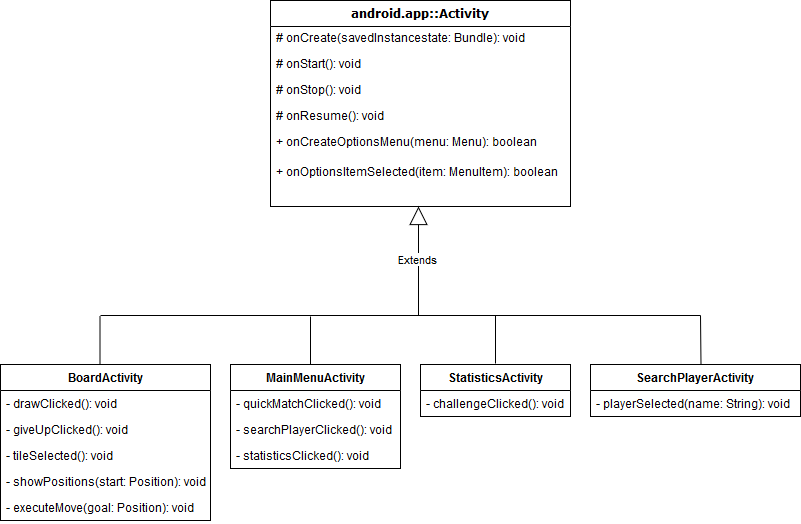
\includegraphics[width=1\linewidth]{Diagramme/ActivityDiagram}
			\captionof{figure}{Activities}
			\label{fig:activities}
		\end{minipage}
	
	\begin{itemize}
			\item \textbf{\Large{android.app.Activity}}
			
			Ist eine einzelne, fokussierte Aufgabe, die der Benutzer ausführen kann. Da fast alle Aktivitäten mit dem Benutzer interagieren, kümmert sich die Activity-Klasse darum, ein Fenster für Sie zu erstellen.\\
			\\			
				\textbf{\large{Methoden}}
				\newline
				\rule{\textwidth}{1pt}
				\begin{description}			
					\item \textbf{\# onCreate(savedInstanceState: Bundle):}\\ Wird aufgerufen, wenn die Aktivität beginnt. Wenn die Aktivität neu initialisiert wird, enthält das Bundle die Daten, die es zuletzt bei SaveInstanceState bereitgestellt hat. Ansonsten ist es \textbf{null}.
					\item \textbf{\# onStart(): }\\ Wird aufgerufen, wenn die Aktivität gestoppt wurde, jetzt aber dem Benutzer wieder angezeigt wird.
					\item \textbf{\# onStop(): }\\ Wird aufgerufen, wenn man für den Benutzer nicht mehr sichtbar sind.
					\item \textbf{\# onResume(): }\\ Wird aufgreufen, damit die Aktivität mit dem Benutzer interagieren kann. 
					\item \textbf{+ onCreateOptionsMenu(menu: Menu): Boolean:}\\ Initialisiert den Inhalt des Standardoptionen-Menüs der Aktivität. Es gibt das Optionsmenü, in dem die Elemente platziert werden sollen. Es gibt true für das angezeigte Menü zurück und bei false wird es nicht angezeigt.
					\item \textbf{+ onOptionsItemSelected(item: MenuItem): Boolean:}\\ Wird aufgerufen, wenn ein Element im Optionsmenü ausgewählt wird. Item ist das ausgewählte Menüelement. Es gibt false zurück, um die normale Menüverarbeitung fortzusetzen und true, um sie dann zu verbrauchen.\\
				\\
				\item \textbf{\Large{BoardActivity}}
			
			Es werden alle Borad-Aktivitäten angezeigt, wie z.B. das Brett.\\
			
			\item \textbf{\Large{MainMenuActivity}}
			
			Es werden alle Menü-Aktivitäten angezeigt, wie z.B. die Knöpfe Sofotrspiel, Spielersuche und Rangliste/Statistik.\\
			
			\item \textbf{\Large{RankingStatisticsActivity}}
			
			Es werden alle Ranglisten und Statistiken-Aktivitäten angezeigt, wie z.B. ein Rangliste mit allen Spielern und den jeweiligen Punkten oder eine Statistik über den Spieler angezeigt.\\
				\end{description}
				\end{itemize}
				
				\newpage	
		\subsubsection{Dialoge}
		\begin{minipage}{\linewidth}
			\centering
			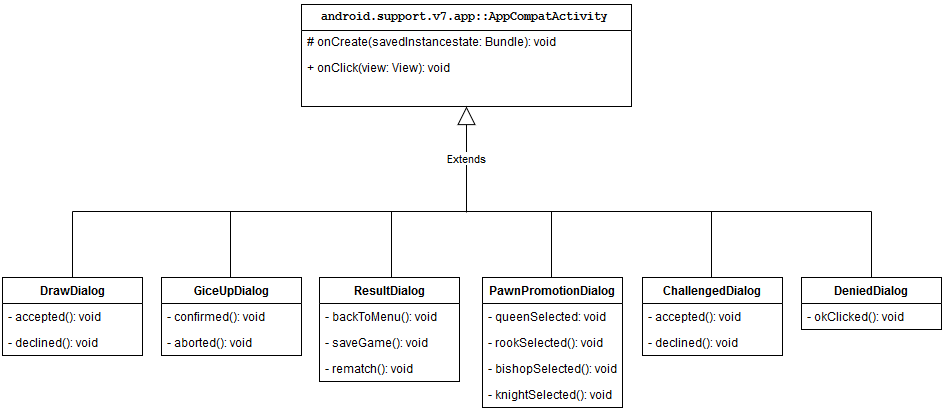
\includegraphics[width=1\linewidth]{Diagramme/DialogDiagram}
			\captionof{figure}{Dialoge}
			\label{fig:dialoge}
		\end{minipage}
		\begin{itemize}
			\item \textbf{\Large{android.app.Activity}}
			
			Die AppComaptActivity wird als Dialog verwendet.\\
			\\			
				\textbf{\large{Methoden}}
				\newline
				\rule{\textwidth}{1pt}
				\begin{description}			
					\item \textbf{\# onCreate(savedInstanceState: Bundle):}\\ Erzeugt die Knöpfe. Wenn die Aktivität neu initialisiert wird, enthält das Bundle die Daten, die es zuletzt bei SaveInstanceState bereitgestellt hat. Ansonsten ist es \textbf{null}.
					\item\textbf{+ onClick(view: View)}:\\ Erzeugt die Fuktionalität eines Konpfes wobei ein AlertiDialog geöffnet wird
					\\
				
					\item \textbf{\Large{DrawDialog}}
			
					Es wird ein Unentschieden-Dialog angezeigt, wie z.B. das Brett.\\
					
					\item \textbf{\Large{GiveUpDialog}}
					
					Es werden alle Menü-Aktivitäten angezeigt, wie z.B. die Knöpfe Sofotrspiel, Spielersuche und Rangliste/Statistik.\\
					
					\item \textbf{\Large{LoginMenuDialog}}
					
					Es werden alle Ranglisten und Statistiken-Aktivitäten angezeigt, wie z.B. ein Rangliste mit allen Spielern und den jeweiligen Punkten oder eine Statistik über den Spieler angezeigt.\\
					
					\item \textbf{\Large{WinnerDialog}}
					
					Es werden alle Menü-Aktivitäten angezeigt, wie z.B. die Knöpfe Sofotrspiel, Spielersuche und Rangliste/Statistik.\\
					
					\item \textbf{\Large{PawnTransformationDialog}}
					
					Es werden alle Ranglisten und Statistiken-Aktivitäten angezeigt, wie z.B. ein Rangliste mit allen Spielern und den jeweiligen Punkten oder eine Statistik über den Spieler angezeigt.\\
				\end{description}
				\end{itemize}
		\newpage
		
		\subsection{ClientSocket}
		\begin{minipage}{\linewidth}
			\centering
			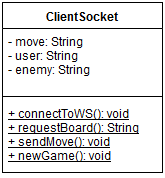
\includegraphics[width=1\linewidth]{Diagramme/ClientSocket}
			\captionof{figure}{ClientSocket}
			\label{fig:ClientSocket}
		\end{minipage}
		\begin{itemize}	
				
			\item \textbf{\Large{ClientSocket}}
		
			Baut eine \gls{WS}-Verbindung zum Server auf.
			Sendet zudem \gls{HTTP}-Anfragen an den Server.
			
			\textbf{\large{Methoden}}
			\newline
			\rule{\textwidth}{1pt}
			\begin{description}
				\item \textbf{+ connectToWS(): void}
				
				Baut eine \gls{WS}-Verbindung zum Server auf. Die App wird über diese Verbindung benachrichtigt, falls der Gegner einen Zug ausgeführt hat.
				
				\item \textbf{+ requestBoard(): String}
				
				Sendet eine GET-Anfrage an den Server, die den aktuellen Brettzustand zurückgibt.
				
				\item \textbf{+ sendMove(move: String): String}
				
				Sendet einen Zug an den Server.  Bekommt eine Meldung, je nachdem, ob der gesendete Zug gültig war.
				
				\item \textbf{+ newGame(opponent: String): String}
				
				Sendet eine Anfrage für die Erstellung eines neuen Spiels. Bekommt eine Meldung, wenn das Spiel erstellt wurde.
				
				\item \textbf{- getUser(): String}
				
				Gibt den Nutzernamen des App-Nutzers zurück.
			\end{description}
		\end{itemize}
		\newpage
		\subsection{Server}
		\begin{minipage}{\linewidth}
			\centering
			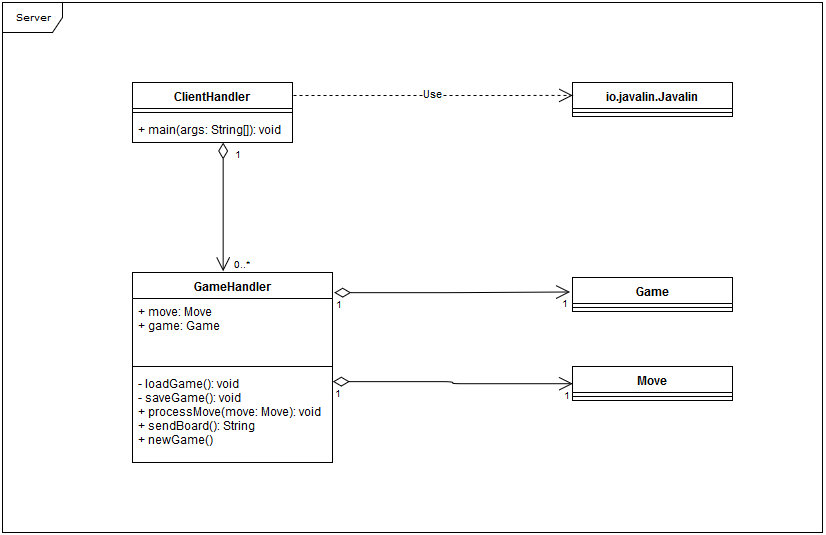
\includegraphics[width=1\linewidth]{Diagramme/Server}
			\captionof{figure}{Server}
			\label{fig:server}
		\end{minipage}
		\begin{itemize}
			\item \textbf{\Large{ClientHandler}}
			
			Verwaltet eingehende Anfragen an den Server.\\
			\\			
			\textbf{\large{Methoden}}
			\newline
			\rule{\textwidth}{1pt}
			\begin{description}
				\item \textbf{+ main(String[] args): void}\\ Die main Methode des Servers. Hier wird der Javalin Server gestartet. Je nach Anfrage wird ein \textbf{GameCreator}, ein \textbf{BoardHandler} oder ein \textbf{MoveHandler} erstellt. \\
				\\
			\end{description} 	
	
			\item \textbf{\Large{GameCreator}}
			
				\textbf{\large{Attribute}}
				\newline
				\rule{\textwidth}{1pt}
				\begin{description}
					\item \textbf{- player1: String}\\
					Spieler 1 des neuen Spiels.
					\item \textbf{- player2: String}\\
					Spieler 2 des neuen Spiels.\\
					\\
				\end{description}	
				\textbf{\large{Methoden}}
				\newline
				\rule{\textwidth}{1pt}
				\begin{description}
					\item \textbf{+ create(player1: String, player2: String)}\\ Erstellt einen neuen Spiel-Eintrag in der Datenbank. Benutzt dazu einen \textbf{DatabaseHandler}.\\
					\\
				\end{description}		
		
			\item \textbf{\Large{BoardHandler}}
			
				\textbf{\large{Attribute}}
				\newline
				\rule{\textwidth}{1pt}
				\begin{description}
					\item \textbf{- board: BoardState}\\
					Aktueller Zustand des Bretts.\\
					\\
				\end{description}	
				\textbf{\large{Methoden}}
				\newline
				\rule{\textwidth}{1pt}	
				\begin{description}
					\item \textbf{+ getBoard(player: String): String}\\ Lädt das entsprechende Spielbrett aus der Datenbank. Verwendet ebenfalls einen DatabaseHandler.\\
					\\
				\end{description}
		
		
			\item \textbf{\Large{MoveHandler}}
				
				\textbf{\large{Attribute}}
				\newline
				\rule{\textwidth}{1pt}
				\begin{description}
					\item \textbf{- move: Move}\\
					Der Zug der überprüft und ausgeführt wird.
					\item \textbf{- board: BoardState}\\
					Das Spielbrett auf dem dieser Zug ausgeführt werden soll.\\
					\\
				\end{description}
				\textbf{\large{Methoden}}
				\newline
				\rule{\textwidth}{1pt}	
				\begin{description}
					\item \textbf{+ processMove(move: Move): BoardState}\\ Laden und Speichern erfolgen wieder über einen \textbf{DatabaseHandler}. Überprüft, ob die Kombination aus Brett und Zug gültig ist. Wendet den Zug an, falls dieser gütlig ist. Speichert das neue Brett ab und benachrichtigt anschließend den Gegner.\\
					\\
				\end{description}
		
		
			\item \textbf{\Large{DatabaseHandler}}
			
				Legt die Methoden fest, die ein \textbf{DatabaseHandler} implementieren muss.\\
				\\				
				\textbf{\large{Methoden}}
				\newline
				\rule{\textwidth}{1pt}
				\begin{description}
					\item \textbf{+ newEntry(player1: String, player2: String): void}\\ Soll einen neuen Datenbankeintrag mit Spieler 1 , Spieler 2 und einem neuen Brett anlegen.
					\item \textbf{+ loadGame(player: String): String}\\ Soll das zum Spieler zugehörige Brett aus der Datenbank laden.
					\item \textbf{+ saveGame(player: String): void} Soll ein Brett wieder in die Datenbank speichern.\\
					\\
				\end{description}
			
		
			\item \textbf{\Large{FirebaseHandler}}
			
				Verwaltet die Verbindung zur Firebase Datenbank.\\
				\\				
				\textbf{\large{Methoden}}
				\newline
				\rule{\textwidth}{1pt}
				\begin{description}
					\item \textbf{+ newEntry(player1: String, player2: String): void}\\	
					Erstellt einen neuen Eintrag mit beiden Spielern und einem neuen Brett.
					\item \textbf{+ loadGame(player: String): String}\\
					Lädt das zum Spieler zugehörige Brett aus der Datenbank.
					\item \textbf{+ saveGame(player: String): void}\\
					Speichert das Brett wieder ab.
				\end{description}
			
			
		\end{itemize}
	\section{Sequenzdiagramm}
	
	\printglossaries
\end{document}